\section{Ridges}

\paragraph*{}
Ridges are brief bright or dark impulses on contrasting background. Differing from step edges in their definition, they also require slightly different method of extraction. We will start the description from the point in which we have just extracted and refined the 1D profile of image brightness, as illustrated in \reffig{RidgesProfile}.

\begin{figure}[h!]
    \begin{subfigure}[b]{\basicWidth}
		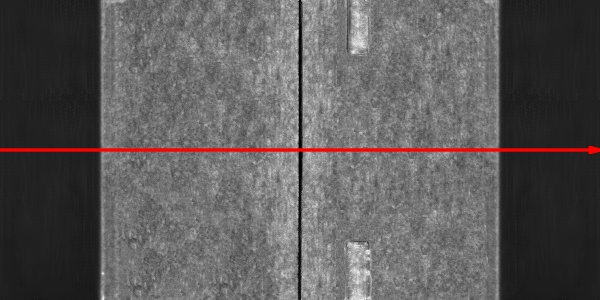
\includegraphics[width=\linewidth]{img/1DEdgeDetection/ridges_scan}
    \end{subfigure}%
    ~
    \begin{subfigure}[b]{\basicWidth}
		\smallProfile{img/1DEdgeDetection/ridges_profile.values}
    \end{subfigure}
    \caption{1D brightness profile of an image with strong ridge in its center.}
    \label{fig:RidgesProfile}
\end{figure}

\subsection{Ridge Operator}

\paragraph*{}
Ridges can be thought of as pairs of step edges of opposite polarity lying extremely close to each other. We could use this observation to propose a simple ridge detector operator adding together results of Forward Difference and Backward Difference operators:
\begin{eqnarray*}
R[i] & = & (S[i]-S[i-1])+(S[i]-S[i+1]) \\
	& = & 2S[i]-S[i-1]-S[i+1]
\end{eqnarray*}

\paragraph*{}
Such operator would be a discreet equivalent of the ridge operator proposed by Canny\cite{Canny86}, it has however two important drawbacks, pointed out by Subirana-Vilanova and Sung\cite{Subirana-VilanovaSung93}:

\begin{itemize}
	\item The operator has non-zero response for step edges, which can easily lead to false-positive errors.
	\item The quality of the detection strongly depends on the ridges having exactly 1 pixel in width, while in reality ridges usually appear as at least slightly wider.
\end{itemize}

\paragraph*{}
Both problems are illustrated by \reffig{RidgesNaiveResponse} - we can notice high impulse response for step edges on the boundary of the object. Moreover, as the ridge in the original image has three pixels in width, it appears in the resulting profile as a pair of consecutive step edges.

\profileFigure
{
	\addProfileData{img/1DEdgeDetection/ridges_naive_operator.values}
}
{Naive ridge detection operator applied to the example profile.}
{RidgesNaiveResponse}

\paragraph*{}
The authors of \cite{Subirana-VilanovaSung93} suggest to solve the problem of high response to step edges by applying each half of the ridge operator separately and using the minimum of two responses.

\[
	R[i] = \min(S[i]-S[i-1],S[i]-S[i+1])
\]

\paragraph*{}
Such form of the operator is already feasible for narrow (one pixel wide) ridges. To successfully detect wider ridges we could define a general operator parametrized by the width of the ridge and the width of the reference margin as follows:

\begin{eqnarray*}
R[i] & = \min( & \\
	& & \overline{S[i..(i+Width)]}-\overline{S[(i-1-Margin)..(i-1)]}, \\
	& & \overline{S[i..(i+Width)]}-\overline{S[(i+1)..(i+1+Margin)])} \\
	& ) &
\end{eqnarray*}

where $\overline{S[a..b]}$ denotes the average of S values between $a$-th and $b$-th element, mutually inclusive.

\paragraph*{}
It should be noted that contrary to edge detection operator which could be applied regardless of the polarity of edges being extracted, our ridge detection operator (because of the minimum function) works specifically for bright ridges. To extract dark ridges, analogous equation with maximum operator should be used.

\paragraph*{}
\reffig{RidgesProperResponse} demonstrates the outcome of using such operator on the example data we consider in this section. The maximum operator suppresses the magnitude of negative values (indicating possible ridge candidates) but amplifies the magnitude of positive values. For clarity the drawing was cropped to negative-y part.

\profileFigure
{
	\addProfileData{img/1DEdgeDetection/ridges_proper_operator.values}
}
{Amended ridge detection operator applied to the example profile.}
{RidgesProperResponse}

\paragraph*{}
Example results of ridge detection performed using such operator are demonstrated in \reffig{RidgesResults}.

\oneFigure
{img/1DEdgeDetection/ridges_result}
{Results of ridge detection.}
{RidgesResults}
{\basicWidth}

\subsection{Post-processing}

\paragraph*{}
All methods of post-processing of the extracted step edge points described in Step Edges section are applicable to ridges. 

\begin{refImpl}
Ridge detection algorithms are implemented in three \studio filters. All of them share common extraction logic, differing only in post-processing method applied to select the final outcome.
\begin{itemize}
	\item \filter{ScanMultipleRidges}{1DEdgeDetection} - returns all of the extracted ridges.
	\item \filter{ScanExactlyNRidges}{1DEdgeDetection} - selects the most prominent set of ridges of given cardinality.
	\item \filter{ScanSingleRidge}{1DEdgeDetection} - wrapper over previous filter which selects the single most prominent ridge.
\end{itemize} 
\end{refImpl}
